\documentclass[11pt]{standalone}
\usepackage{amssymb}
\usepackage{amsmath}
\usepackage[no-math]{fontspec}
\usepackage{unicode-math}
\usepackage{libertinus}
\usepackage{pgf,xcolor}
\usepackage{tikz}
\usetikzlibrary{arrows.meta, backgrounds}
\usepackage{pgfplots}
\pgfplotsset{compat=newest}

\definecolor{my_darkgray}{HTML}{484949}
\definecolor{my_lightgray}{HTML}{F3F4F4}
\definecolor{my_darkblue}{HTML}{005A94}
\definecolor{my_lightblue}{HTML}{CCDEE9}
\definecolor{my_yellow}{HTML}{FFEC7F}
\definecolor{my_red}{HTML}{E60000}
\definecolor{my_orange}{HTML}{E87846}

\begin{document}

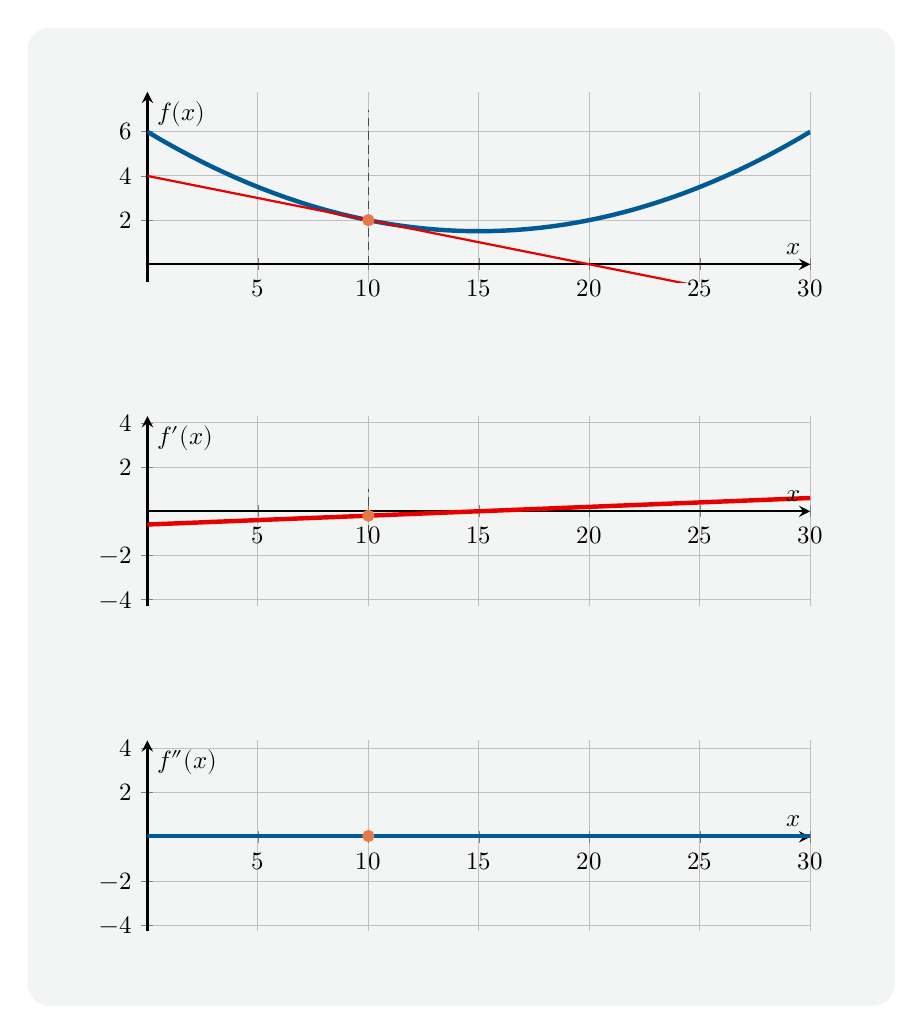
\begin{tikzpicture}[
    show background rectangle,
    background rectangle/.style={fill=my_lightgray, rounded corners=8pt},
    inner frame sep=0.8cm
]

% ======================================================
% TOP PANEL: original function f(x) and tangent at x=10
% ======================================================
\begin{axis}[
    name=plotF,
    at={(0,6cm)},
    anchor=center,
    width=10cm,
    height=4cm,
    axis lines = center,
    xlabel = {$x$},
    ylabel = {$f(x)$},
    xmin=0, xmax=30,
    ymin=0, ymax=7,
    grid = both,
    axis equal,
    axis line style={thick},
    ticklabel style={font=\small},
    label style={font=\small},
]

% original function f(x) = 0.02 x^2 - 0.6 x + 6
\addplot[
    draw=my_darkblue,
    ultra thick,
    samples=300,
    domain=0:30
]
{0.02*x^2 - 0.6*x + 6};

% tangent line at x0 = 10:
% f(10) = 2, f'(10) = -0.2,
% tangent y = 2 - 0.2 (x - 10) = 4 - 0.2 x
\addplot[
    draw=my_red,
    thick,
    domain=0:30
]
{4 - 0.2*x};

% point on the curve at x0 = 10, f(10) = 2
\addplot[
    only marks,
    mark=*,
    mark size=2pt,
    draw=my_orange,
    fill=my_orange
]
coordinates {(10,2)};

% vertical alignment line
\addplot[
    draw=my_darkgray,
    densely dashed,
    very thin
]
coordinates {(10,0) (10,7)};

\node[anchor=south west, font=\small\bfseries, my_darkgray]
at (rel axis cs:0.02,0.98) {Height profile $f(x)$ and its tangent at $x=10$};

\end{axis}

% ==============================================
% MIDDLE PANEL: first derivative f'(x)
% ==============================================
\begin{axis}[
    name=plotFp,
    at={(plotF.south west)},
    anchor=north west,
    yshift=-1.7cm,
    width=10cm,
    height=4cm,
    axis lines = center,
    xlabel = {$x$},
    ylabel = {$f'(x)$},
    xmin=0, xmax=30,
    ymin=-1, ymax=1,
    grid = both,
    axis equal,
    axis line style={thick},
    ticklabel style={font=\small},
    label style={font=\small},
]

% first derivative f'(x) = 0.04 x - 0.6
\addplot[
    draw=my_red,
    ultra thick,
    samples=300,
    domain=0:30
]
{0.04*x - 0.6};

% point at x0 = 10, f'(10) = -0.2
\addplot[
    only marks,
    mark=*,
    mark size=2pt,
    draw=my_orange,
    fill=my_orange
]
coordinates {(10,-0.2)};

% vertical alignment line
\addplot[
    draw=my_darkgray,
    densely dashed,
    very thin
]
coordinates {(10,-1) (10,1)};

\node[anchor=south west, font=\small\bfseries, my_darkgray]
at (rel axis cs:0.02,0.98) {Slope function $f'(x)$};

\end{axis}

% ==============================================
% BOTTOM PANEL: second derivative f''(x)
% ==============================================
\begin{axis}[
    name=plotFpp,
    at={(plotFp.south west)},
    anchor=north west,
    yshift=-1.7cm,
    width=10cm,
    height=4cm,
    axis lines = center,
    xlabel = {$x$},
    ylabel = {$f''(x)$},
    xmin=0, xmax=30,
    ymin=0, ymax=0.12,
    grid = both,
    axis equal,
    axis line style={thick},
    ticklabel style={font=\small},
    label style={font=\small},
]

% second derivative f''(x) = 0.04
\addplot[
    draw=my_darkblue,
    ultra thick,
    samples=2,
    domain=0:30
]
{0.04};

% point at x0 = 10, f''(10) = 0.04
\addplot[
    only marks,
    mark=*,
    mark size=2pt,
    draw=my_orange,
    fill=my_orange
]
coordinates {(10,0.04)};

% vertical alignment line
\addplot[
    draw=my_darkgray,
    densely dashed,
    very thin
]
coordinates {(10,0) (10,0.12)};

\node[anchor=south west, font=\small\bfseries, my_darkgray]
at (rel axis cs:0.02,0.98) {Second derivative $f''(x)$ as constant slope change};

\end{axis}

\end{tikzpicture}

\end{document}